% Nama kelompok : kelompok 4
% Kelas : D4 TI 1A
% Anggota :
% Muhammad Dzihan Al-Banna	: 1174095
% Yusuf Al-Qardhawi			: 1174085
% Nurresky					: 1174019
% Daffa Naufali Pratama		: 1174010







Artikel tentang Storage
\ref{storage}
\begin{figure}[ht]
\centerline{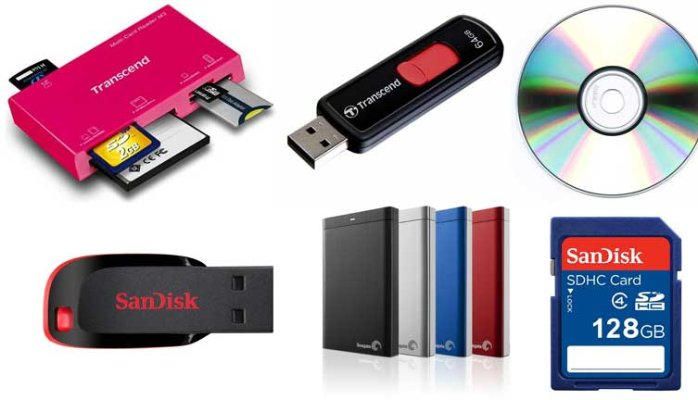
\includegraphics[width=1\textwidth]{figures/storage.jpg}}
\caption{contoh storage}
\label{storage}
\end{figure}





\section{Pengertian Storage}

Storage merupakan salah satu perangkat yang digunakan untuk menyimpan hasil dari pemprosesan data dan sistem operasi. Storage biasanya terdapat didalam komputer,storage ini bisa disebut juga dengan secondary storage.
Storage device dibagi menjadi dua bagian yaitu internal dan eksternal. internal storage device contohnya seperti Hard Disk. Internal Storage ini terdapat dalam komputer. sedangkan Eksternal Storage Device adalah suatu penyimpanan data tambahan pada komputer yang terletak diluar komputer,contohnya Hard Disk Eksternal,Flash Disk,Floppy Disk atau biasa kita sebut disket.
dalam suatu artikel menyebutkan bahwa storage merupakan penyimpanan \cite{weiser1999personal}

\section{Sejarah Storage}
Pada tahun 1725 ada seorang tokoh bernama basile bounchon yang merancang sebuah media untuk menyimpan data.Bouchon menggunakan kertas berforasi untuk menyimpan pola yang digunakan pada kain.Namun penemuannya itu baru dipatenkan pada tahun 1884 oleh Herman Hollerith.Penemuan Bouchon ternyata sangat berguna,terbukti,penemuannya digunakan selama lebih dari 100 tahun hingga pertengahan 1970.Penemuannya ini diberi nama punch card,sebuah media penyimpanan yang memiliki 90 kolom.Namun,jumlah data yang tersimpan dalam media tersebut sangatlah kecil dan fungsi utamanya bukan untuk menyimpan data melainkan untuk menyimpan pengaturan atau setting untuk mesin yang berbeda.Pada tahun 1864 Alexander Bain menemukan penemuan baru,paper tape yang biasanya digunakan untuk mesin faksimil atau telegram,dia modifikasi sehingga dapat menyimpan data.Penemuannya ini dinamakan punch tape,ada beberapa keunggulan yang didapat dari punch tape ini.Punch tape dapat menyimpan data lebih signifikan dibandingkan punch card.Barulah pada tahun 1946 ada sebuah perangkat penyimpanan yang dapat menyimpan data dengan mencantumkan ukuran tertentu,yaitu selectron Tube.Selectron Tube merupakan awal format memori komputer selectron.Dulunya harga selectron tube ini sangat mahal dan langja di pasaran.Kemudian pada tahun 1970 banyak orang yang sudah mengenal kaset dan menggunakannya untuk menyimpan data.Kaset ini merupakan terobosan yang sangat bagus karena lebih memudahkan pengguna untuk menyimpan data.Kaset ini bisa menyimpan data mulai dari 700kb sampai 1mb.
Seiring berkembangnya zaman dan ilmu pengetahuan,maka storage device ini terus berkembang dan semakin banyak pula ruang yang disediakan untuk menyimpan  data.Untuk pertama kalinya ada hard drive yang dapat menyimpan data sampai 500GB.Tiap tahunnya selalu saja ada kemajuan dan semakin bertambah besar ruangan yang disediakan untuk menyimpan data ini.Sampai saat ini tentu semakin banyak jenis-jenis storage device dan semakin mudah juga para pengguna menggunakannya,bahkan ukurannya juga ada yang kecil sehingga mudah untuk dibawa kemana-mana.

\section{Macam-macam storage Device}

1.Hard Disk Drive

Hard disk merupakan salah satu media penyimpanan data pad komputer yang terdiri dari kumpulan piringan magnetis keras dan berputar,serta komponen elektronik lainnya.Hard disk menggunakan piringan datar yang disebut dengan platter yang pada kedua sisinya dilapisi dengan suatu material yang dirancang agar bisa menyimpan informasi secara magnetis.Platter ini berputar dengan kecepatan tinggi.Setiap permukaan pada platter menampung sati milyar bit data,setiap platter menyimpan informasi dalam lingkaran-lingkaran yang disebut dengan track.Tiap track dipotong-potong lagi menjadi beberapa bagian yang disebut dengan sector.Seperti yang disebutkan di \cite{wahyudi2005mengenal}

2.Floppy Disk

Floppy disk drive adalah suatu perangkat penyimpanan yang ada didalam komputer yang dapat menyimpan data dalam kapasitas rendah.Dalam satu komputer bisa terdapat dua floppy sekaligus,tapi biasanya hanya terdapat satu floppy saja yaitu floppy A. Semua jenis floppy dilengkapi dengan unit mekanis seperti driver disk dan head positioner,Drive disk inilah yang membuat disk berputar.selain dapat menyimpan data didalam disket,floppy disk juga dapat untuk boating komputer.Seperti yang disebutkan di \cite{horie1987floppy}
3.Compact Disk

Compact disk ini biasa kita singkat CD adalah sebuah piringan kompak dari jenis piringan optik yang dapat menyimpan data.Compact Disk ini dapat menyimpan data sebesar 700 MB.Untuk membaca CD ini, alat yang diperlukan adalah CD DRIVE.CD ini bersifat hanya dapat dibaca tetapi tidak dapat ditulis,tetapi pada perkembangan terkini CD ini dapat ditulis.Seperi yang disebutkan di \cite{ernst1998turtles}

4.Flashdisk

Flashdisk adalah suatu perangkat penyimpanan yang dibuat perangkat dengan minimalis dengan ukuran kecil dengan kapasitas tertentu. Flashdisk ini dibuat dengan
mudah dan simpel karena perangkat ini sangat mudah sekali dipakai dan dibawa kemana saja. Selain itu komponen flashdisk ini mendukung usb 2.0 dan usb 3.0 tergantung
versi base yang dibuat oleh perusahaan flashdisk tersebut. Flashdisk ini mempunyai kapasitas pertama kali diluncurkan dengan ukuran 1 GB dan seiring waktu berjalan
Kapasitas ini semakin diperbesar oleh penemu flashdisk ini hingga 2 tb saat ini. Kecepatan Reading Flashdisk ini berkisar antara 1Mb/s sampai dengan 12Mb/s.Seperti yang disebutkan di \cite{aini2010mengukur}

Flashdisk ini dikatakan bahwa flash yang artinya melakukan read and scan, dan disk artinya perangkat storage. Jadi Flashdisk ini bekerja secara Read and Scan untuk
menganalisa isi perangkat tersebut apabila anda menghubungkan sesuai driver usb sesuai dukungan devices. Harga Flashdisk ini dikalangan masyarakat relatif murah
kisaran antara Rp 30ribu sampai dengan Rp 100ribu.Selain memudahkan pengguna,terkadang ukuran flashdisk yang kecil membuat penggunanya lupa menyimpan,bahkan ada yang sampai tercuci di mesin cuci.

5.Memory Card

Memory Card atau kartu memory adalah sebuah alat yang digunakan untuk menyimpan data.Ukuran memory card ini bermacam-macam,mulai dari 126 MB sampai 16 GB.Kartu memori ini ukurannya kecil,tapi dapat menyimpan data dengan ukuran yang besar,terdapat beberapa jenis ukuran memori,tetapi biasanya kartu memori mempunyai ukuran standar bit digital yaitu 16MB,32MB,64MB,128MB,256MB dan seterusnya kelipatan dua.Bukan hanya data dokumen tetapi memori juga bisa menyimpan gambar,video ataupun audio.Ukuran dari memory card sangat kecil,sehingga banyak sekali orang yang kehilangan memory,untuk mengantisipasinya,sebaiknya memory card jangan terlalu sering dilepas dari perangkat anda.

6.Magnetic Tape

Magnetik Tape adalah suatu media perekam yang terdiri dari gulungan tape halus yang terbuat dari bahan magnetis,karena itulah sering disebut dengan tape magnetis,bentuknya menyerupai tape yang biasa kita pasang diradio zaman dulu.Akan tetapi fungsinya memang seperti tape musik zaman dulu karena tape magnetis ini dapat merekam suara juga.Namun kendala pada tape jenis ini adalah mudah rusak,apalagi jika gulungan magnetisnya sampai berantakan,seperti tape kaset radio.


\section{keunggulan dan kekurangan storage internal}

Storage internal mempunyai keunggulan tersendiri daripada storage eksternal,karena storage internal tersimpan didalam maka tidak mungkin bagi storage internal ini menghilang secara tidak sengaja dari perangkat anda.Dalam komputer anda biasanya terdapat ruang penyimpanan seperti data E,data C dan data D,sebenarnya itu merupakan salah satu keunggulan storage internal yang kuat untuk dipartisi hingga beberapa bagian.Jika anda memindahkan file pun akan lebih cepat menggunakan storage internal karena mempunyai kemampuan write and read yang lebih cepat.Dan yang paling penting storage internal ini mempunyai umur yang panjang atau lebih tahan lama.

\section{keunggulan dan kekurangan storage eksternal}

Storage eksternal yang mempunyai ukuran lebih kecil tentu memudahkan pemiliknya untuk membawanya kemana-mana,namun karena ukurannya kecil,storage eksternal ini sering hilang.Walaupun bentuknya kecil,storage eksternal ini mempunyai kapasitas yang tak kalah besar daripada storage internal bahkan beberapa storage eksternal bisa mempunyai kapasitas melebihi storage internal.Storage eksternal ini terletak diluar,jadi walaupun rusak,kamu dapat dengan mudah menggantinya.Walaupun begitu kemungkinan besar kehilangan atau lupa menaruh storage jenis ini sangat besar sekali dikarenakan ukurannya yang kecil.Selain itu storage eksternal ini juga cepat rusak karena banyak sekali kemungkinan yang bisa membuat storage eksternal ini rusak seperti tercuci dan berkarat.Terlalu sering digunakan juga bisa menjadi penyebab storage eksternal ini lebih cepat rusak.Karena terletak diluar,maka proses mengcopy file melalui storage eksternal ini sangat lambat,ini disebabkan kemampuan write and ride nya yang kurang cepat.Seseuai dengan harganya yang lebih murah,sudah tentu storage eksternal ini mempunyai kekurangan lebih banyak daripada storage eksternal dari segi ketahanannya dan kemampuannya,tetapi storage jenis ini juga mempunyai keunggulan yang tidak ada di storage internal.

\section{Kesimpulan}

Storage device adalah media penyimpanan data dengan berbagai jenis,bentuk dan ukuran.Jenis dari storage terbagi dua,yaitu storage device internal dan storage device eksternal,storage device internal mempunyai keunggulan yaitu tahan lama dan lebih cepat saat membaca data dan aman karena terletak didalam pc maka storage internal tidak mudah hilanag.Sedangkan storage eksternal yang terletak diluar sangat rawan terjadi kehilangan karena bentuknya yang kecil,storage eksternal juga mudah rusak karena banyak kemungkinan yang terjadi pada storage jenis ini seperti tercuci ataupun jatuh.Kekurangan yang lain dari storage ini adalah lambat pada saat proses pembacaan data oleh komputer.masing-masing storage mempunyai keunggulan tersendiri dan bentuknya pun beragam,ada yang besar dan ada juga yang sangat kecil.Untuk ruang penyimpanan itu sendiri bermacam-macam mulai dari ukuran beberapa byte sampai tera.Sampai saat ini masih dicari storage yang lebih memanjakan para penggunanya agar lebih aman,mudah dibawa,tidak mudah hilang tetapi dengan kapasitas yang besar.



